\documentclass[10pt,a4paper,twoside]{article}

\usepackage[T1]{fontenc}
\usepackage[latin1,utf8]{inputenc}

\usepackage{lmodern}

\usepackage[pdftex]{graphicx} 

\usepackage[tracking=true]{microtype}
               
                               
\usepackage{amsmath,amssymb,amsthm}
\usepackage{xfrac}
\usepackage{mathrsfs}
\usepackage{mathtools}
\usepackage{grffile}  

\usepackage{bbm} %for use of identity-matrix
\usepackage{dsfont}

\usepackage[]{subfigure}
\usepackage{wrapfig}
\usepackage{multicol}

\usepackage{verbatim}
\usepackage{setspace}

\usepackage{color}
\usepackage[]{hyperref}
\usepackage{listings}

\usepackage{accents}
\usepackage{textcomp}
\usepackage{multirow}
\usepackage{booktabs}
\usepackage{float}

\usepackage[numberedbib]{apacite}
\bibliographystyle{apacite}
\usepackage[flushleft]{threeparttable}
\usepackage{tabulary}
\usepackage{indentfirst}


\usepackage{geometry}
\geometry{a4paper,left=30mm,right=25mm, top=20mm, bottom=25mm}

\usepackage{fancyhdr}
\pagestyle{fancy}
\fancyhf{}
\rhead{André Crescenzo}
\lhead{\small{Computer-aided Design of Bio-inspired Nanoporous Silica Materials}}
\lfoot{\today}
\rfoot{\thepage}

\usepackage{abstract}
\usepackage{authblk}



\title{Computer-aided Design of Bio-inspired Nanoporous Silica Materials}
\author[1,2]{André Crescenzo\thanks{ Corresponding author.\\ Email: \ \texttt{andre.crescenzo.2014@uni.strath.ac.uk}}}
\author[1]{Alessia Centi\thanks{ Email: \ \texttt{alessia.centi@strath.ac.uk}}}
\author[1]{Miguel Jorge\thanks{Email: \ \texttt{miguel.jorge@strath.ac.uk}}}
\affil[1]{Department of Chemical and Process Engineering, University of Strathclyde}
\affil[2]{Departamento de Engenharia Química da Escola Politécnica, Universidade de São Paulo}
\renewcommand\Authands{ and }
\date{\today \\
\begin{abstract}
\textbf{Aim:} Finish my job!\\
\textbf{Conclusion:}Repeating the results is not drawing a conclusion.
\begin{tabular}
& \textbf{Keywords}: Latex$\cdot$ Bibtex  $\cdot$ Scientific Paper $\cdot$ More Scientific Papers $\cdot$ More Scientific Papers  $\cdot$ More Scientific Papers $\cdot$ More Scientific Papers $\cdot$ More Scientific Papers $\cdot$ More Scientific Papers 
\end{tabular}
\end{abstract}}

\pagenumbering{roman}

\begin{document}
%\doublespace
\begin{titlepage}

\newcommand{\HRule}{\rule{\linewidth}{0.5mm}} 

\center 
 
\begin{figure*}[ht!]
	
\includegraphics[width=1 \textwidth]{./images/StrathLogo}
\end{figure*}


\textsc{\LARGE University of Strathclyde}\\[1.5cm] 
\textsc{\Large Department of Chemical \& Process Engineering}\\[0.5cm] 
\textsc{\large M.Eng Chemical \& Process Engineering 18530}\\[0.5cm] 


\HRule \\[0.4cm]
{ \huge \bfseries Computer-aided Design of Bio-inspired Nanoporous Silica Materials}\\[0.4cm] % Title of your document
\HRule \\[1.5cm]
 

\begin{minipage}{0.4\textwidth}
\begin{flushleft} \large
\emph{Author:}\\
André \textsc{Crescenzo} 
\end{flushleft}
\end{minipage}
~
\begin{minipage}{0.4\textwidth}
\begin{flushright} \large
\emph{Supervisors:} \\
Miguel \textsc{Jorge} \\ 
Alessia \textsc{Centi} \\
Carlos F. \textsc{Rangel}
\end{flushright}
\end{minipage}\\[4cm]

{\large \today}\\[3cm] % Date, change the \today to a set date if you want to be precise


\vfill 

\end{titlepage}
\addtocontents{toc}{~\hfill\textbf{Page}\par}
\section{Summary}
\setcounter{page}{1}
...
\vfill
\newpage

\setcounter{tocdepth}{3}
\tableofcontents



\vfill
\newpage

\section{Acknowledgements}

\textit{...}

\vfill
\newpage

\pagenumbering{arabic}
\section{Introduction}
%%%%%%%%%%%%%%%%%%%%%%%%%%%%%%%%%%%%%%%%%%%%%%%%%%%%%%%%%%%%%%%%%%%%%%%%%%%%%%%%%%%%%%%%%%%%%%%%%%%%%%
%A good introduction is a clear statement of the problem or project and the reasons for studying it. 
%This information should be contained in the first few sentences.										
%Give a concise and appropriate background discussion of the problem									
%and the significance, scope, and limits of the work. Outline what has been done						
%before by citing truly pertinent literature, but do not include a general survey of					
%semirelevant literature. State how your work differs from or is related to work						
%previously published. Demonstrate the continuity from the previous work to yours.					
%The introduction can be one or two paragraphs long. Often, the heading								
%“Introduction” is not used because it is superfluous; opening paragraphs are usually introductory	
%%%%%%%%%%%%%%%%%%%%%%%%%%%%%%%%%%%%%%%%%%%%%%%%%%%%%%%%%%%%%%%%%%%%%%%%%%%%%%%%%%%%%%%%%%%%%%%%%%%%%%
%clear statement of the problem + reasons for studying it\\
%  background discussion\\
%  what has been done by others(cite works)\\
%  how mine differs from the others\\
%  how it relates to the others\\
%  significance of the work\\
%  scope of the work\\
%  limts of the work\\
%  continuity?(maybe silica interactions...)\\

Molecular Dynamics (MD) and Monte Carlo (MC) are powerful tools to simulate molecular interactions of surfactants in solvent systems, allowing a deeper understanding of their self-assembly process \cite{mjsilica}. This process results in several types of surfactant mesoscale conformations that are specially useful to design bio-inspired silica materials \cite{bioinsp}. With the addition of silica, these structures behave as scaffolds to mesoporous or nanoporous structures that are maintained even after surfactant removal, silica oligomer polymerization and calcination \cite{silica1}.
A vast range of silica materials are examples of this phenomena, such as MCM-41 as reported by \citeA{mcm}, SBA-15 \cite{sba}, MSU-V \cite{msuv} and many others, in which the self-assembled structure depends on the type of surfactant, concentration of the substances involved and synthesis conditions such as temperature and pH. It should be noted that most of the experimental methods used to obtain data are based on observation and interpretation of final silica structure by using X-ray diffraction (XRD) and transmission electron microscopy (TEM). It follows that initial self-assembled conformations are predicted as a reflex of the final results and little is known about the mechanistic of this process. However, with MD simulations it is possible to observe and analyse these initial steps of self-assembly and predict, with more accuracy, properties and frameworks provided by surfactants \cite{lipid}.

%  background discussion\\
%  what has been done by others(cite works)\\
On the other hand, a major concern is that even though MD uses sophisticated software prepared to simulate systems with thousands of atoms, using all capacities of hardware available, such as high-speed multi-core processors in conjunction with GPUs designed specifically to process data from arrays \cite{gromacs}, they can hardly achieve long time horizons and are commonly limited to a few microseconds depending on the size of the system. For this reason, several techniques have been developed to optimize the performance of the simulations such as coarse-grain methods \cite{mjsilica}. The basic idea of this technique is to fit parameters of atom groups with similar properties in a bigger "bead", which includes atomic masses and electrostatic charges lumped in approximated values. For example, given a simulation of an arbitrary surfactant with a long hydrophobic tail, it is possible to merge three or four carbon atoms (and its hydrogen atoms) in groups since they have similar hydrophobic properties, by this means reducing the number of particles in the system and speeding up the simulation. 

%  how mine differs from the others\\
%  how it relates to the others\\
In order to provide molecular topologies to simulations software packages several force-fields, for example MARTINI \cite{martini}, uses Lennard-Jones potentials fitted to a range of pre-defined bead types to describe coarse-grain models. Furthermore, not only intramolecular beads are possible, but also intermolecular beads can be specified, such as multiple solvent molecules merged in a single bead or ions surround by water molecules. Previous works conducted by \cite{mjsilica} with this method recreated a model of surfactant in the presence of silica with explicit water that was successful in describing rod-like self-assembly structures detected on MCM-41 materials, demonstrating the capacities of up-scaling this type of systems. Nevertheless, solvent presence demands most of the computational resources, hence  implicit solvent scheme has been the focus of many studies \cite{gromacs}.

Different concepts have been applied to develop a suitable model for implicit solvents; For example, \citeA{drymartini} developed the Dry MARTINI force-field by modifying parameters of its predecessor, in such manner that solvent interactions became incorporated in these values and then solvent beads are no longer necessary. Another method, described by \citeA{magic} is able to recreate an implicit solvent system from interaction potentials generated from a bottom-up approach, that means by using an all-atoms simulation to generate parameters for the coarse-grain model. It is supposed  that these approximated potentials can be refined iteratively by this systematic method based on averages calculated from Monte Carlo simulations. 
During this process thermodynamic changes originated from solvent interaction with amphiphilic molecules or even electrostatic interactions can be incorporated in the potentials derived, therefore providing a flexible methodology to up-scale systems allowing the simulation of mesoscale self-assembly structures using coarse-graining.

%  significance of the work\\
%  scope of the work\\
%  limts of the work\\
The experiments presented in this work are an attempt to develop a  method to upscale silica-surfactant interactions \cite{silica1} from the atomistic model to a mesoscale model with the advent of this later coarse-grain technique. The methodology applied to reach the desired model is based on the MagiC software package \cite{magic} that in conjunction with a MD simulation software, in this case GROMACS \cite{gromacs}, will provide a suitable approximation to self-assembly of amphiphilic molecules. Further explanations of the process are described in the Experimental Methods section. For the scope of this project, a bolaamphiphilic molecule called 1,12-diaminododecane (DMDD) has been chosen as surfactant because, as seen in previous research by \citeA{msuv}, it self-assembles in multilamelar vesicles that in the presence of a silica precursor are capable of generating a mesoporous structure with remarkable properties. In order to validate this structure formation and framework formation for silica oligomers, a coarse-grain approximation is a suitable option since amphiphilic molecules interaction with solvents can be described efficiently with potentials derived from the chosen methodology \cite{myproj}. As a final objective at the end of this project, an implicit water coarse-grain model for DMDD and Silica will be generated and properly validated based on MD simulations and thermodynamic properties, in order to provide a satisfactory approximation of self-assembled silica-surfactant structures in mesoscale. 
%  continuity?(maybe silica interactions...)\\


\section{Theoretical Basis}
This work is based on two molecular simulation techniques. The former, called Molecular Dynamics, accounts for integration of Newton forces in order to describe positions and velocities of particles in the system. The latter, called Monte Carlo method, is a powerful statistical tool based on stochastic inputs to measure properties from many systems, in this case molecular systems in thermodynamic equilibrium. In the following sections the mechanism behind each technique will be described, including additional explanations on how they are applied in simulation software.
\subsection{Simulation Methods}
\subsubsection{Molecular Dynamics simulation}

Molecular Dynamics is a simulation method that originates from the dynamic nature of atomic interactions. Generally, a system of atoms can be treated as a multi-particle system ruled by Newton's Law \cite{umd}. Considering a system with $\mathcal{N}$ atoms, for each $i$th particle of the system the following differential equation will determine its dynamic behaviour:
\begin{equation}
m_i\dfrac{\,d^2\vec{r}_i(t)}{\,dt^2} = \vec{F}_i(t)
\label{eqn:newton}
\end{equation}

Where $\vec{r} = (x,y,z)$ is the position vector and $F = (F_x, F_y, F_z)$ are the force components. Therefore, for this $\mathcal{N}$ particle system, it is necessary to solve $3\mathcal{N}$ differential equations in order to fully describe it analytically at any $t$. Since any molecular system involves an enormous number of molecules, solving these equations analytically is impracticable and simulation methods are necessary. The derivative terms need to be numerically calculated and as soon as simulation efficiency is a major concern, a suitable approximation to the second derivative of position is the Taylor's expansion, taking the x coordinate as an example, for a given $\Delta t$ is:
\begin{equation}
x(t+\Delta t) = x(t) + \Delta t \dfrac{\,dx(t)}{\,dt} + \dfrac{1}{2!}{\Delta t}^2 \dfrac{\,d^2x(t)}{\,dt^2} + \dfrac{1}{3!}{\Delta t}^3 \dfrac{\,d^3x(t)}{\,dt^3} +  \mathcal{O}(\Delta t^4)
\label{eqn:taylor1}
\end{equation}
\begin{equation}
x(t-\Delta t) = x(t) - \Delta t \dfrac{\,dx(t)}{\,dt} + \dfrac{1}{2!}{\Delta t}^2 \dfrac{\,d^2x(t)}{\,dt^2} - \dfrac{1}{3!}{\Delta t}^3 \dfrac{\,d^3x(t)}{\,dt^3} +  \mathcal{O}(\Delta t^4)
\label{eqn:taylor2}
\end{equation}
\begin{equation}
\dfrac{\,d^2x(t)}{\,dt^2} = \dfrac{x(t+\Delta t) - 2 x(t) + x(t-\Delta t)}{{\Delta t}^2} +  \mathcal{O}(\Delta t^2)
\label{eqn:dx2}
\end{equation}

Hence, by neglecting the error of order $\mathcal{O}(\Delta t^2)$, it is possible to use equations (\ref{eqn:newton}) and (\ref{eqn:dx2}) to derive the called "Verlet method" where position and velocity vectors for each $i$th atom on next step ($t+\Delta t$) are calculated using previous and current step:
\begin{equation}
\vec{r}_i(t+\Delta t) = 2 \vec{r}_i(t) - \vec{r}_i(t-\Delta t) + \dfrac{{\Delta t}^2}{m_i}\vec{F}_i(t)
\label{eqn:verletr}
\end{equation}
\begin{equation}
\vec{v}_i(t) =  \dfrac{\vec{r}_i(t+\Delta t) - \vec{r}_i(t-\Delta t)}{2{\Delta t}}
\label{eqn:verletv}
\end{equation}

In order to improve accuracy of the Verlet method, another approach can be made by accounting for a new force term in the velocity. This term is calculated from the updated position vector, and this improved velocity term is used to calculate the new position in the next step, creating a more precise step cycle with more stability \cite{satoh}. This set of equations is called "Velocity Verlet method" and it is described as:
\begin{equation}
\vec{r}_i(t+\Delta t) = \vec{r}_i(t) + \vec{v}_i(t)\Delta t + \dfrac{\vec{F}_i(t)}{2m_i}{\Delta t}^2
\label{eqn:vverletr}
\end{equation}
\begin{equation}
\vec{v}_i(t+\Delta t) = \vec{v}_i(t) + \dfrac{\vec{F}_i(t+\Delta t)+\vec{F}_i(t)}{2m_i}\Delta t
\label{eqn:vverletv}
\end{equation}

As a final variation for Verlet method one can derive the "Leap frog method", in which one considers half-step when calculating the velocity term. Even though the use of this technique leads to a more stable and accurate behaviour when compared to Verlet method, it is noticeable that velocity and position are not in the same time steps, therefore it is not possible to calculate the total energy at a given $t$, just kinetic or potential energy separately \cite{umd}. By applying first-order derivatives with half-steps, one can obtain the following equations:
\begin{equation}
\vec{r}_i(t+\Delta t) = \vec{r}_i(t) + \vec{v}_i(t+\sfrac{\Delta t}{2})\Delta t
\label{eqn:leapfrogr}
\end{equation}
\begin{equation}
\vec{v}_i(t+\sfrac{\Delta t}{2}) = \vec{v}_i(t-\sfrac{\Delta t}{2}) + \dfrac{\vec{F}_i(t)}{m_i}\Delta t
\label{eqn:leapfrogv}
\end{equation}

The force term for each step is a key factor to define whether Molecular Dynamics are realistic or not. They are strictly related to the force-field adopted to describe molecular interactions, since they provide parameters to specify intra and intermolecular potentials from which forces can be calculated at any system configuration. Eventually, as seen in innovative methods such as the used on this project, the potential values can also be provided by tables generated specifically for each molecular interaction, explanations about this technique will be given on further sections (See Section \ref{subsubsec:magic}). Molecular dynamics technique enables the use of thermostats and barostats to control dynamic behaviour of temperature and pressure of the system, recreating different types of thermodynamic ensemble. Hence, at equilibrated states, system properties can be obtained as a temporal average of instantaneous values and those averages can be compared to real experimental data in order to validate simulations.

\subsubsection{Monte Carlo simulation}
Monte Carlo is  a simulation method based on the statistical probability of existence of a system at thermodynamic equilibrium. The equilibrium condition happens when the free energy reaches a minimum by calculating the energy for each particle's microscopic state. Given a system of $ \mathcal{N}$ particles, temperature $T$ and volume $V$ (thus it can be denoted as a canonical ensemble), it is possible to assume that  the Helmholtz free energy of this system is:
\begin{equation}
A = U - TS
\label{eqn:freeE}
\end{equation}
where $S$ is the entropy and $U$ is the internal energy, meaning that not only a minimum in free energy can arise from a minimum in total energy, but also an increase in entropy of the system can contribute to this energy minimization. A system can be described by a group of coordinates, in this case for clarity, a group of distance vectors $\lambda = (	\vec{r}_1,\vec{r}_2, \ldots, \vec{r}_\mathcal{N} )$ from system origin. For an arbitrary $\lambda$ the probability of a single particle of the system to statistically occupy that position is described by a probability distribution function \cite{satoh}:
\begin{equation}
\rho(\lambda) = \dfrac{\exp{\left(-\dfrac{U(\lambda)}{kT}\right)}}{\displaystyle \int_V \dots   \int_V \exp{\left(-\dfrac{U(\lambda)}{kT}\right)}\,d\vec{r}_1 \,d\vec{r}_2 \ldots \,d\vec{r}_\mathcal{N} }
\label{eqn:rho}
\end{equation}

If the system configuration is generated with a considerable number of microstates that satisfies this probability, then the final configuration will have a real physical meaning. But, as soon as it is almost impossible to define an analytical solution to this equation when $\mathcal{N}$ is too large, another method became necessary to use Monte Carlo simulations in molecular dynamics. The Metropolis method \cite{metropolis} allowed the use of Monte Carlo technique by introducing the following concept: given 2 different microstates, the probability to change from state 1 to 2 is defined by:

\begin{equation}
 P_{1\mapsto2} = \left\{
\begin{array}{c l}     
    1 & for \ \frac{\rho(\lambda_2)}{\rho(\lambda_1)}\geqslant1\\
    \dfrac{\rho(\lambda_2)}{\rho(\lambda_1)} & for \ \frac{\rho(\lambda_2)}{\rho(\lambda_1)}<1
\end{array}\right.
\label{eqn:metrop}
\end{equation}

 Therefore, the integral term in eq.(\ref{eqn:rho}) vanishes and it is clear to observe that when $U(\lambda_1) \geqslant U(\lambda_2)$ the system will certainly change to this new microstate since it has lower energy, however in the case of $U(\lambda_1) < U(\lambda_2)$ the system has a certain probability of changing to this new microstate indicating an increase of entropy in the system. So, by applying stochastic inputs for particle displacements and acceptance values for eq.(\ref{eqn:metrop}), with a large number of Monte Carlo steps the system will eventually reach a minimum in free energy.
  Moreover, when this system reaches equilibrium it is possible to calculate accurately microstate dependent properties via ensemble averages. That means with $n$ samples of Monte Carlo steps, the average of a $ \xi $ property can be obtained by:
 
 \begin{equation}
\left\langle \xi\right\rangle  = \displaystyle \sum_{i=1}^{n} \dfrac{\xi_i}{n}
\label{eqn:average}
\end{equation}

It is important to notice that Monte Carlo simulations do not consider dynamic properties of the system such as kinetic energy, and therefore only Molecular Dynamics can account for such things \cite{satoh}. Finally, now that both molecular simulation methods have been introduced it is possible to proceed to an overview of both simulation software used on this project. Together they can unite the benefits of both simulation methods, in order to recreate a suitable coarse-grain model for Molecular Dynamics.
\subsection{Software Description}
\subsubsection{About GROMACS}

 GROMACS (\textbf{Gro}ningen \textbf{Ma}chine for \textbf{C}hemical \textbf{S}imulations) \cite{gromanual} is a Molecular Dynamics and energy minimization software created at the University of Groningen (the Netherlands), and currently has been developed and updated by Royal Institute of Technology (Sweden) and Uppsala University (Sweden). GROMACS is a widely used tool in the branch of computational chemistry because it is flexible and efficient. Its flexibility comes from the capacity of simulating multiscale molecular models, from atomistic to mesoscale depending on topology described by the user. The efficiency originates from the computational optimisation, by this meaning not only that GROMACS can achieve impressive simulation speed in large systems using supercomputing or clusters, but also it can run small simulations in any ordinary computer with great performance.
 
 In order to interpret interatomic interactions, that means forces between each pair of atoms, GROMACS uses input files called Topologies in which the user can describe almost any molecule using force fields or tabulated potentials. Data given in this description includes information regarding atoms' type, mass and charge. Moreover, it includes a detailed description of each bond, angle and dihedral for the molecule. There are several Force-fields available for usage depending on the desired objective of the simulation, their role is to be a database that describes interaction potentials. Hence their applicability is suitable to almost any system from all-atoms to coarse-grain descriptions, but it is entitled to the user to choose the most appropriate to obtain a realistic model.
 
  When dealing with simulations of complex systems, realism means more computational power expended trying to achieve it \cite{satoh}, therefore a major concern is how to achieve longer time horizons without loosing precision. A good example is the Lennard-Jones potential for Van der Waals forces, used by OPLS-AA Force-field \cite{opls}, which is the one chosen for all-atom simulations in this project. This type of potential approximation for a given atom $i$ in relation to atom $j$ is defined simply by two parameters  $\epsilon$ and $\sigma$ as it can be seen in Eq.\ref{eqn:ljpot}:

\begin{equation}
\mathcal{U}_{LJ}(r_{ij}) = 4\epsilon_{ij}\left(\left( \dfrac{\sigma_{ij}}{r_{ij}}\right)^{12} - \left( \dfrac{\sigma_{ij}}{r_{ij}}\right)^6\right) 
\label{eqn:ljpot}
\end{equation}

 \begin{figure}[ht]
  \begin{center}
	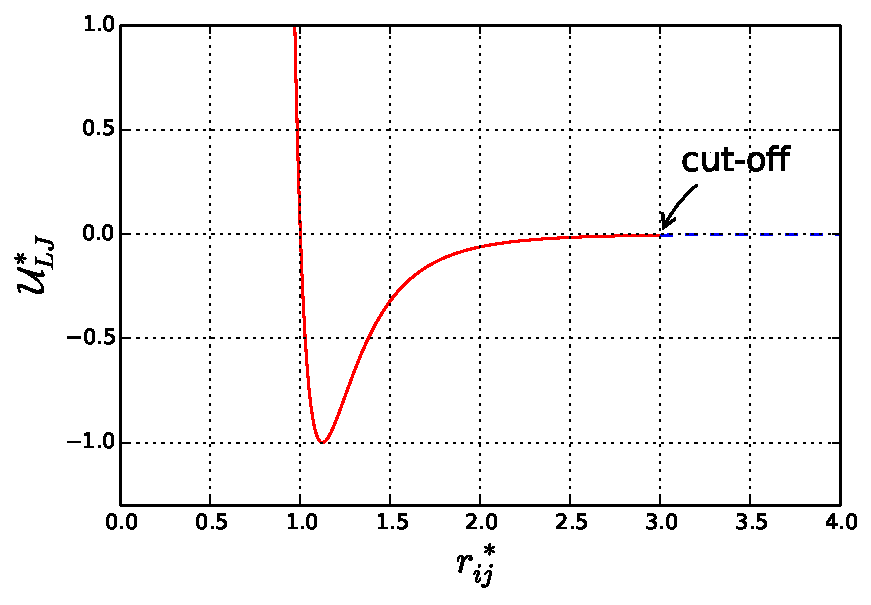
\includegraphics[width=0.6 \textwidth]{./graphs/lj}
	\caption{Example of Lennard-Jones Potential (with reduced units). For this plot $\epsilon = 1$ and $\sigma = 1$ }
	\label{gfx:ljg}
	\end{center}
	\end{figure}

Where the forces used in Molecular Dynamics equations come from the gradient of this potential for each pair of particles:
\begin{equation}
\vec{F}_{ij} = \nabla\mathcal{U}_{LJ}(r_{ij}) = \left( \dfrac{\partial\mathcal{U}_{LJ}(r_{ij})}{\partial x}\hat{x} + \dfrac{\partial\mathcal{U}_{LJ}(r_{ij})}{\partial y}\hat{y}+\dfrac{\partial\mathcal{U}_{LJ}(r_{ij})}{\partial z}\hat{z}\right) 
\label{eqn:ljf}
\end{equation}

For every simulation time-step, GROMACS recalculates bonded potentials from topology, non-bonded potentials from the summation of Lennard-Jones potentials and Coulomb potentials. As shown in Figure (\ref{gfx:ljg}) if $r_{ij} \rightarrow \infty$ $\Rightarrow$ $\mathcal{U}_{LJ} \rightarrow 0$ and a similar behaviour occurs for Coulomb forces. Hence, GROMACS generates a neighbour list of atoms determined by a cut-off radius for each particle, by this means avoiding having to spend a lot of computational power calculating numbers with negligible value. Moreover, this feature allows the use of periodic boundary conditions that recreate a continuous media environment for simulation boxes bigger than  two times the cut-off radius, since each particle cannot interact with itself. 

Although speed efficiency is a concern, it is not the only preoccupation. In fact, it is also necessary to control environment variables such as temperature and pressure, in order to maintain the simulation within physical limits, which demands computational resources. GROMACS is capable of using three types of thermostat: Berendsen, v-rescaling and Nosé-Hoover and three types of barostat: Berendsen, Parrinello-Rahman and MTTK \cite{gromanual}. Furthermore, other computational expensive technique is the use of Particle-mesh Ewald (PME) summation method \cite{ewald} to deal with long-range electrostatic interactions, which is indispensable in ionic environments. All these tools makes GROMACS not only fast but also reliable for Molecular Dynamics simulation, moreover this project will as well demonstrate the capacity of this software to simulate realistic multi-scale molecular models.
  
\subsubsection{About MagiC}
\label{subsubsec:magic}
MagiC is a software package developed by \citeA{magic}, which is a systematic method to generate coarse-grain models from all-atomic simulations using Iterative Boltzmann Inversion (IBI) and Inverse Monte Carlo (IMC). As described in Figure (\ref{Fig:magic}), this method consists of a three step process where the input is the trajectory file of an equilibrated all-atoms simulation from GROMACS, and outputs are a set of tabulated potentials and a Topology for a coarse-grained model that uses these potentials to run Molecular Dynamics simulations using GROMACS. 
 \begin{figure}[ht]
  \begin{center}
	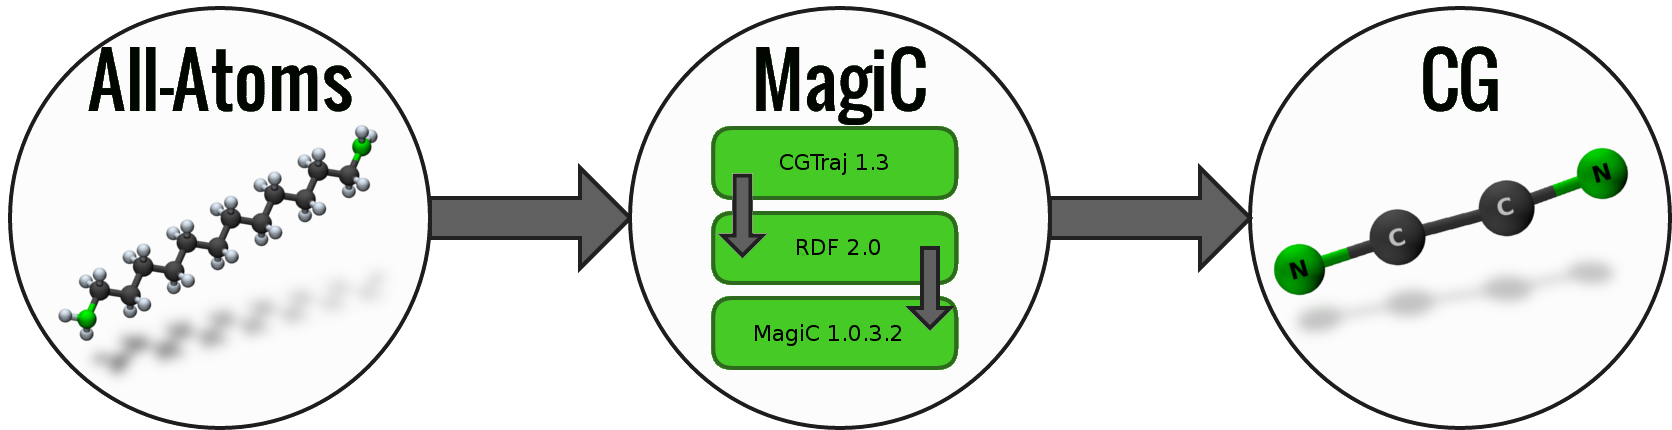
\includegraphics[width=1 \textwidth]{./images/magic}
	\caption{Graphical representation of Magic's systematic process. The central circle represent the process itself while the other two are input and output. The green boxes indicates each step inside MagiC process. }
	\label{Fig:magic}
	\end{center}
	\end{figure}

 The first step uses "CGtraj 1.3" (MagiC package utility written in Fortran 90) \cite{magicmanu}, where the trajectory of the all-atoms simulation is recalculated based on a bead mapping described by the user. Basically, it analyses the group of atoms in each bead and assigns the position of this bead as the center of mass, charge as summation of all charges and mass as summation of atomic masses, thus giving as output a representation of the input system as if it was an "ideal" coarse-grain model. Next, this rewritten trajectory is used as input to rdf-2.0  (MagiC package utility written in Python) \cite{magicmanu}, where several reference Radial Distributions Functions are created for each bond, angle and pairwise intermolecular interaction, as specified by the user. These reference RDFs in conjunction with the coarse-grain topology are the  inputs to the MagiC kernel (MagiC package utility written in Fortran 90) \cite{magicmanu}, which is the key step of the process, where the final output might be a suitable coarse-grain model ready for GROMACS simulation.
 
 The kernel is where the actual Inversion process occurs, as schematised in Figure (\ref{Fig:kernel}). Whether using IMC or IBI, a couple of millions of Metropolis Monte Carlo steps are simulated using a set of trial potentials to create several samples of averaged thermodynamics properties. Then, these averages are applied in the equations of the chosen inversion method in order to refine the trial potentials that will be used in the next inversion step.
 \begin{figure}[ht!]
  \begin{center}
	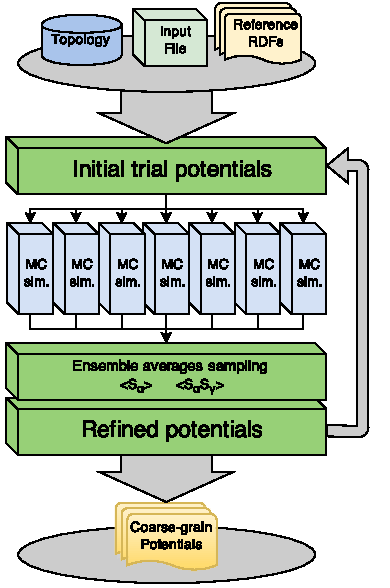
\includegraphics[width=0.50\textwidth]{./images/magiccore}
	\caption{MagiC kernel work-flow scheme}
	\label{Fig:kernel}
  \end{center}
\end{figure}
 
 The Iterative Boltzmann Inversion is a reasonable methodology to apply in the initial iterations, since it has fast convergence. The process derives from probability distribution function (Eq.(\ref{eqn:rho})), thus for a pairwise particle interaction, the relationship between the reference RDF and Potential Mean Force (PMF) enables the use of an iterative method shown in Eq.(\ref{eqn:ibi}) \cite{ibi}:
   \begin{equation}
\mathcal{U}^{(i+1)}(r) = \mathcal{U}^{(i)}(r) - \eta k_B T \ln{\left(\dfrac{\rho^{(i)}(r)}{\rho_{ref}(r)}\right)}
\label{eqn:ibi}
\end{equation}

 Where $\eta$ is a regularization parameter to avoid excessive variations. For a system in a canonical ensemble, temperature will be constant, hence the potential is corrected for each iteration using the $\rho_{ref}(r)$ calculated from reference RDF in comparison to $\rho^{(i)}(r)$ from  RDF generated by Metropolis Monte Carlo simulation. Although this method is efficient to achieve small deviations from references, it does not guarantee that the generated potential represents one that will reproduce a behaviour similar to atomistic model because IBI does not consider cross-correlation terms between bonds and angles \cite{magic}.   
 
 Regarding the Inverse Monte Carlo process, it follows the methodology described by \citeA{imc}. Given a Hamiltonian, that means the total energy of the system:
 \begin{equation}
\mathcal{H}(q) = \displaystyle \int \mathcal{U}_\alpha\mathcal{S}_\alpha(q) \,d\alpha
\label{eqn:hami}
\end{equation}

For pair interactions, the degree of freedom $q$ in Eq.(\ref{eqn:hami}) becomes the distance $r$ between a pair of atoms. Therefore, for a real system the Hamiltonian would be the summation of an infinite set of $\mathcal{U}_\alpha$. However, a good approximation for numerical methods is to assume a cut-off radius $r_{\mathsf{cut}}$, where potentials no longer have relevant value after this point. One can define a $\Delta r = \dfrac{r_{\mathsf{cut}}}{\mathcal{M}}$, obtaining $\mathcal{M}$ subdivisions and thus a finite set of  $\mathcal{U}_{\alpha}$ in which $\mathcal{S}_\alpha$ is the number of pairs within  interval $[r_\alpha,(r_\alpha + \Delta r)]$. Since $\mathcal{S}_\alpha$ is function of $\mathcal{U}$, one can derive the following Taylor expansion:

 \begin{equation}
\Delta\left\langle\mathcal{S}_\alpha\right\rangle = \sum_{\phi=\alpha}^\mathcal{M}\dfrac{\partial\left\langle\mathcal{S}_\alpha\right\rangle}{\partial\mathcal{U}_\phi}\Delta\mathcal{U}_\phi + \mathcal{O}({\Delta\mathcal{U}_\phi}^2)
\label{eqn:inv1}
\end{equation}
 \begin{equation}
\dfrac{\partial\left\langle\mathcal{S}_\alpha\right\rangle}{\partial\mathcal{U}_\phi} = \dfrac{ \left\langle\mathcal{S}_\alpha\right\rangle\left\langle\mathcal{S}_\phi\right\rangle - \left\langle\mathcal{S}_\alpha\mathcal{S}_\phi\right\rangle}{k_B T}
\label{eqn:inv2}
\end{equation}

For each inversion step $k$, Monte Carlo simulations are run using a set of potentials $\mathcal{U}_{\alpha}^{(k)}$, then as explained previously it is possible to calculate ensemble averages of the cross-correlation terms ${\left\langle\mathcal{S}_\alpha\mathcal{S}_\phi\right\rangle}^{(k)}$ and averages $\left\langle\mathcal{S}_\alpha\right\rangle^{(k)}$, $\left\langle\mathcal{S}_\phi\right\rangle^{(k)}$. At this point, the reference RDFs become useful for inverse Monte Carlo. Since this method deals with pairwise interactions the values of $\mathcal{S}_\alpha$ and $\rho(r)$ are directly proportional following the rule $\mathcal{S}_\alpha^{*}= \rho(r_\alpha)\Delta r $ \cite{magic} because both measure the quantity of one type of coarse-grain bead in relation to another. Hence, by using $\Delta\left\langle\mathcal{S}_\alpha\right\rangle = \left\langle\mathcal{S}_\alpha\right\rangle^{(k)} - \mathcal{S}_\alpha^{*}$  in conjunction with Eq.(\ref{eqn:inv1}) and Eq.(\ref{eqn:inv2}) and neglecting the error $\mathcal{O}({\Delta\mathcal{U}}^2)$ the potential correction for next step $\Delta\mathcal{U}_\alpha^{(k)}$ can be obtained and finally potentials are updated using the following  equation:
 \begin{equation}
\mathcal{U}_\alpha^{(k+1)}= \mathcal{U}_\alpha^{(k)}+\Delta\mathcal{U}_\alpha^{(k)}
\label{eqn:potup}
\end{equation} 

All of the previous methods described rely on a considerably large amount of Monte Carlo simulation steps. That is due to the fact that the closer the set of potentials gets to solution, the harder it becomes to distinguish between statistical noise and a suitable potential correction. For this reason, as it can be seen in Figure (\ref{Fig:kernel}), MagiC has a built-in capacity of running parallel Monte Carlo simulation, which enables the user to reach the order of billions of simulation steps in a feasible timespan. Moreover, there is not a unique solution for a given RDF \cite{ibi} and eventually the solution can possible diverge at a certain point. Therefore, a satisfactory result depends on analysis of all outputs from inversion steps in order to guarantee convergence. Further explanations regarding functionalities and parameters for MagiC and GROMACS will be provided in the next section.  
\section{Methods Description} 

The main objectives of the experiments of this project can be characterized in three stages: the first is to develop and simulate a suitable model for the silica oligomers and the surfactant in an atomistic scale considering a high pH system. Secondly, the aim is to use MagiC software package to develop potentials for the coarse-grain model proposed using a variety of techniques to improve efficiency of the process. Lastly, the focus will be the evaluation and validation of the self-assembly structures simulated using the coarse-grain models that were generated from the previous experiments.

\subsection{Atomistic Molecular Model}

 A initial concern for the atomistic simulations was the design of the water, surfactant and silica molecules. Beginning with the water molecule, the model used was the TIP4P water (Figure (\ref{Fig:atomistic}a)) created by \cite{tip4p} which is a widely used water model that uses OPLS-AA forcefield \cite{opls} parameters. For the DMDD surfactant, a model was created with the aid of co-workers in OPLS-AA forcefield which increases the reliability of the atomic interactions with the water models, since they use the same forcefield. This surfactant model includes 3 variations as a result of the high pH environment, because as described by \cite{hheads} the hydrophilic Nitrogen head receives an extra hydrogen thus in a solution it may be found the Neutral DMDD molecule (DMDDn), the Single charged DMDD molecule (DMDDs) and the Double charged DMDD molecule (DMDDd). Since atomistic simulations need to be preferably set in a neutral charge environment, an inert anionic Bromide counter-ion was selected to equilibrate the charges.
 
   \begin{figure}[ht!]
  \begin{center}
	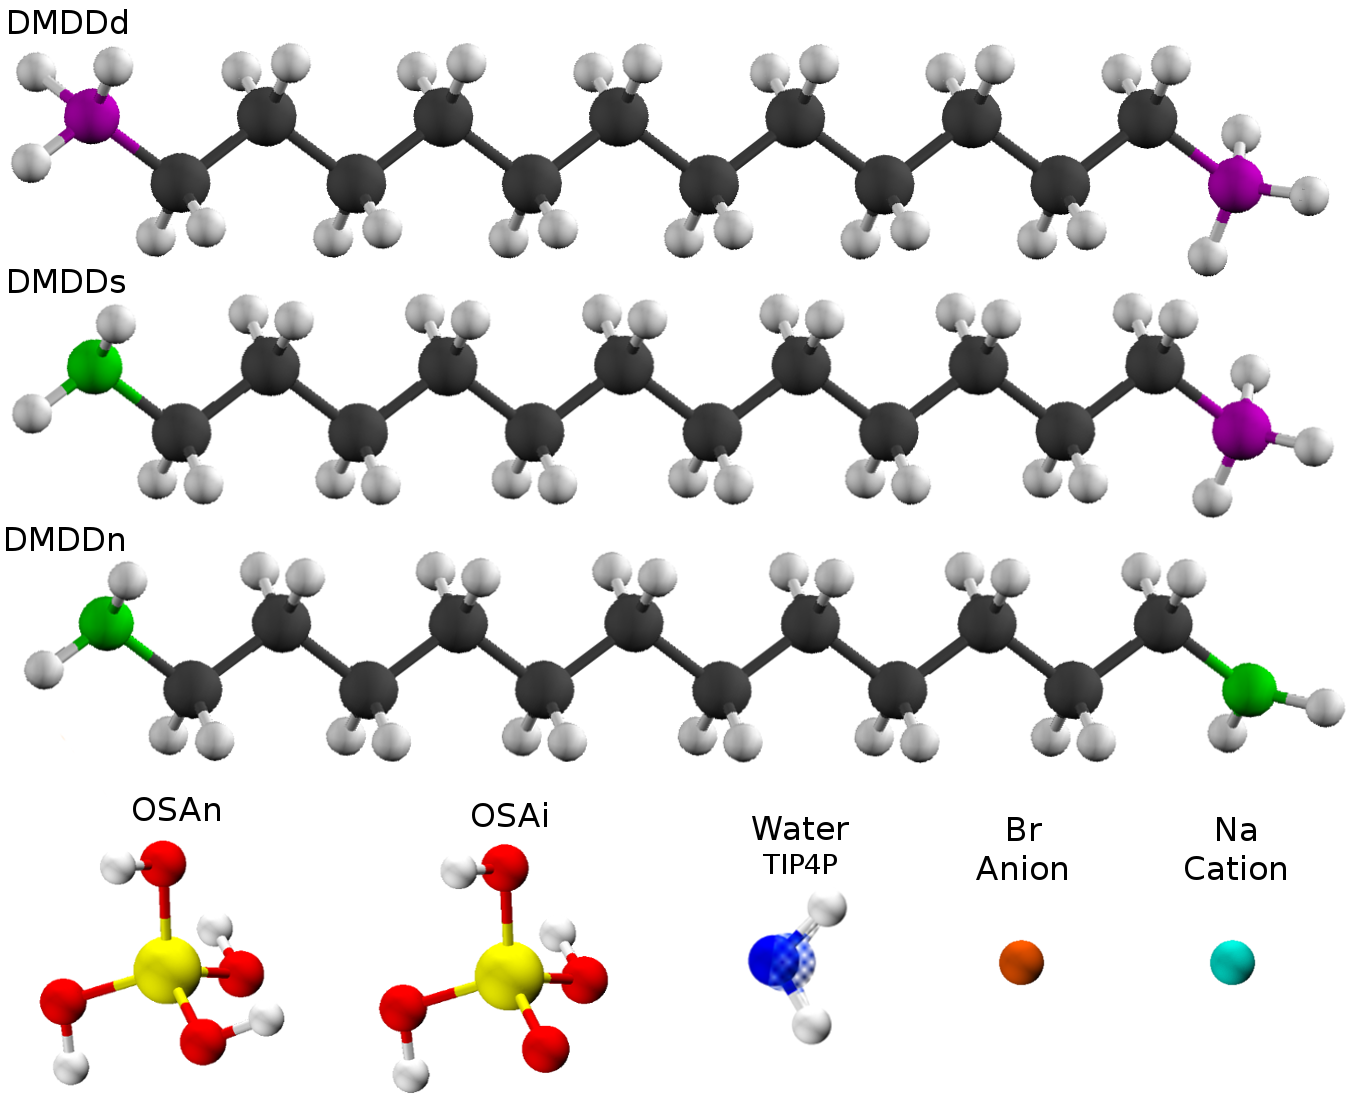
\includegraphics[width=1\textwidth]{./images/molsAA}
	\caption{Graphical representation of the Atomistic models.}
	\label{Fig:atomistic}
  \end{center}
\end{figure}

When it comes to the description of the silica model, it is important to notice that the in solution substances should be treated differently from pure liquid silica precursor. As described in \cite{msuv} the silica precursor tetraethoxysilane (TEOS = $Si(OCH_2CH_3)_4$) is mixed in solution in a ratio of 1:2 in relation to the DMDD surfactant, that means in an atomistic level, one silica to each surfactant head.  However, due to high pH condition a substitution process that might occur in TEOS where it is forced to replace its Ethanol ramifications by hydrogen atoms forming an temporary unstable substance, the orthosilic acid (OSA). As stated by \cite{mjsilica} this unstable silica oligomer is the major representative of the silica portion in the system at early moments in solution state, which in later stages may interact with surfactant structures and polymerise around them in a variety of configurations, turning into a nanoporous and highly organized silica structure. For the scope of this project only the orthosilic acid model will be considered, since the simulations will take place during the formation of the surfactant self-assembly structure which occurs in the early moments of the solution stabilization. Therefore, as it can be seen in Figure (\ref{Fig:atomistic}c) it is possible to consider two principal representations of the orthosilic acid: the neutral molecule (OSAn) and the ionized molecule (OSAi). Similarly to Bromide, cationic Sodium counter-ion will be used to equilibrate the system charge.

\subsection{Atomistic Simulation}

Regarding the composition of each simulation box, the main idea was to work upon the pH value of the solution. The fact of having multiple molecular models allows the creation of simulation boxes with a varying pH, in which each one represent a different stage of deprotonation, that means the higher the number of molecules with missing hydrogen the higher the pH that is represented on the system. It is difficult to determine exactly what is the number of molecules of each type to reach an specific pH, since the molecular types which are deprotonated should vary dynamically \cite{phsol}. This means that even when the ratio of deprotonated and protonated molecules is in an adequate value to represent a certain pH, it might not be possible to guarantee that an specific molecule will remain at the same level of deprotonation  at all times. If a molecule stays at the same state during the whole simulation it will be not representing the desired pH in the system, instead it could create an ambiguity where different regions of the box may represent a different pH value.

 There are several techniques such as represented in work done by \cite{dynph} which are capable to recreate the dynamic behaviour of the pH in solution, which probably can aid to obtain a more accurate results in when it comes to the self-assembled structures in an atomistic level. However, the adoption of such methods goes far beyond the scope of this project's main objectives, and instead in order to maintain the system with a less complex structure only high pH values were represented in simulation boxes. The types of boxes that were chosen used a single state of the molecule to represent a pseudo-high pH solution, because most of them are extreme cases that may not exist in reality but they are good approximations of real systems.

 In previous works, the main subject of study was the DMDDn model, because even though it represent the most extreme case in which all polar heads are deprotonated, indicating a very high pH, it still a feasible approach to real high pH solution and furthermore provides the advantage of not presenting coulomb forces in the coarse-grain model. However, when the silica precursor is introduced in the system it might be unrealistic to assume that the OSA model will ionize all its hydrogens, since it only polymerizes in further stages after the interaction with the surfactant. Hence, the adopted model was the OSAi molecular type that when used together with DMDDn still a system with elevated pH but slightly reduced when compared to pure surfactant solution, since it has non-ionized hydrogens. For this kind of systems two approaches were adopted in order to recreate the simulation boxes. The first method was to randomly insert all molecules inside the box at adequate ratios. The second was to use simulation boxes that were generated based in DMDDn simulations that already had been equilibrated into a layer just by removing the water and putting the right amount of OSAi and then resolvating the box. The specific number of molecules of each type is described in Table (\ref{tab:atombox}), furthermore the implications concerning the use of both methods of box creation will be discussed in Section (\ref{sec:atmbxdiss}).
 
 The second molecular model chosen to represent the surfactant was DMDDs. It was chosen because not only it represents a mid-state between protonation and deprotonation in the polar heads, but also it presents differentiated behaviour when compared to the previous model due to coulombic interactions within the assembled layer. Moreover, the DMDDs simulation boxes can be considered as slightly elevated pH systems when used in conjunction with ionic silica model, since it has just only one ionized head extra per surfactant. In the case of DMDDs, two types of systems were studied: one containing only DMDDs surfactant with Bromide counter-ions to equilibrate the charges, and another with DMDDs and OSAi using Sodium as counter-ion. All boxes were generated using by random placement of the molecules, to ensure whether it occurs layer self-assembly of surfactant or not in both cases, and as the same information about the composition is shown in Table (\ref{tab:atombox}).
 
 \begin{table*}[ht!] 
  \centering
\begin{threeparttable}

  \caption{Table generated by Excel2LaTeX from sheet 'Sheet1'}

    \begin{tabular}{rrrrrr}
    \toprule
    Model & Depth & Width & Angle & Factor 1 & Factor 2 \\
	& (mm) & (mm) & (°)  &  &  \\
    \midrule
    111   & 1,00  & 1,50  & 10\tnote{a}   & 357.921 & 532.289 \\
    112   & 1,00  & 1,50  & 15   & 382.379 & 567.234 \\
    113   & 1,00  & 1,50  & 20   & 383.863 & 569.600 \\
    121   & 1,00  & 2,00  & 10   & 398.199 & 590.473 \\
    122   & 1,00  & 2,00  & 15   & 486.306 & 710.483 \\
    123   & 1,00  & 2,00  & 20   & 430.330 & 636.471 \\
         \midrule
          &       &       & Sum: & 12.138.966 & 17.932.100 \\
    \bottomrule
    \end{tabular}%
    \begin{tablenotes}
    	\item[a] This should be cited with a \citeA{magic}
    	\item[b] And this is another note
    \end{tablenotes}
  \label{tab:atombox}%
\end{threeparttable} 
\end{table*}

It is noticeable that most atomistic boxes have a different concentration. This fact derives from the idea of providing flexibility to the coarse grained model, because they will be used as references to the coarse-grain model. The analysis of the results from previous experiences \cite{myproj}, it is possible to observe that the coarse-grain model can represent and adapt to different apparent concentrations, this fact also means that the coarse-grain potentials obtained from these atomistic simulation boxes contains a certain degree of similarity between them, at least when it refers to the position of the peaks and valleys. Therefore, having multiple similar concentrations within a short range can only benefit the final result obtained since flexibility is a desirable property. Another important point highlight is the box size. For all cases we have two ranges of size: the first is a small box with side bigger than the DMDD molecule (about $16 \ \AA$) used to obtain initial short range potentials; and a big size box with side at least over $40 \ \AA$ to obtain long range potentials. A more detailed explanation about the difference of long range and short range potentials will be given in Section (\ref{expMAGIC})

The simulation boxes generated for all experiments were created using "genbox" (GROMACS package utility) following a standard procedure in order to ensure the consistency of the experiments, moreover all the atomistic simulations that were used as reference for coarse-graining process were run in NPT ensemble. In order to reach this NPT condition, all boxes received an energy minimization step in order to avoid system blow-up due to possible extreme potential energy spots created during box generation. That is because during random displacement of molecules some of them could overlap others and then cause a destabilization of the system. Afterwards, an equilibration step was necessary to reach the desired initial temperature and pressure conditions for the MD simulation. During equilibration, temperature coupling was kept at $298\ K$ using a v-rescaling thermostat \cite{vtstat} with time constant of $0.01\ ps$ and pressure coupling was kept at $1\ bar$ using a Berendsen barostat \cite{berend} with time constant of $0.5\ ps$.  Every equilibration simulation was run for $200\ ps$ with time step of $0.5\ fs$ using leap-frog algorithm.



%all atom boxes 
%-ne+si
%-dmdds+osa
%(-alessia's box )?
%
%magic process
%ne-si
%-coloumb
%-non coulomb
%dmdds+osa
%-coloumb
%-non coloumnb
%
%multi-state tech
%-derivation
%-comparisson
%
%(cg alessia's box)?
%
\section{Results and Discussion}
\section{Conclusion} 
\section{Nomenclature} 
   \begin{tabulary}{1.0\textwidth}{LCL}
   $k_B$ & & Boltzmann's Constant\\
   $C_n$ &   & Molar concentration of species n ($mM$) \\
   \end{tabulary}

\bibliography{./biblio/biblio}
\vfill
\newpage
\section{Appendix}
\label{sec:appendix}
\setcounter{page}{1}
%\begin{equation}
%E_c=\frac{1}{2}mv^2
%\label{eqn:bua}
%\end{equation}
%
%\begin{table*}[ht!] 
%  \centering
%\begin{threeparttable}
%
%  \caption{Table generated by Excel2LaTeX from sheet 'Sheet1'}
%
%    \begin{tabular}{rrrrrr}
%    \toprule
%    Model & Depth & Width & Angle & Factor 1 & Factor 2 \\
%	& (mm) & (mm) & (°)  &  &  \\
%    \midrule
%    111   & 1,00  & 1,50  & 10\tnote{a}   & 357.921 & 532.289 \\
%    112   & 1,00  & 1,50  & 15   & 382.379 & 567.234 \\
%    113   & 1,00  & 1,50  & 20   & 383.863 & 569.600 \\
%    121   & 1,00  & 2,00  & 10   & 398.199 & 590.473 \\
%    122   & 1,00  & 2,00  & 15   & 486.306 & 710.483 \\
%    123   & 1,00  & 2,00  & 20   & 430.330 & 636.471 \\
%    131   & 1,00  & 2,50  & 10   & 441.735 & 654.499 \\
%    132   & 1,00  & 2,50  & 15   & 460.925 & 681.645 \\
%    133   & 1,00  & 2,50  & 20   & 469.115 & 693.700 \\
%    211   & 1,25  & 1,50  & 10   & 374.784 & 557.029 \\
%    212   & 1,25  & 1,50  & 15   & 399.053\tnote{b} & 591.402 \\
%    213   & 1,25  & 1,50  & 20   & 411.377 & 609.042 \\
%    221   & 1,25  & 2,00  & 10   & 415.050 & 615.336 \\
%    222   & 1,25  & 2,00  & 15   & 430.991 & 638.237 \\
%    223   & 1,25  & 2,00  & 20   & 455.857 & 673.613 \\
%    231   & 1,25  & 2,50  & 10   & 472.885 & 698.958 \\
%    232   & 1,25  & 2,50  & 15   & 484.567 & 715.341 \\
%    233   & 1,25  & 2,50  & 20  & 497.320 & 733.923 \\
%    311   & 1,50  & 1,50  & 10   & 385.110 & 572.665 \\
%    312   & 1,50  & 1,50  & 15   & 406.144 & 602.130 \\
%    313   & 1,50  & 1,50  & 20   & 480.613 & 706.960 \\
%    321   & 1,50  & 2,00  & 10   & 490.910 & 722.194 \\
%    322   & 1,50  & 2,00  & 15   & 513.846 & 754.804 \\
%    323   & 1,50  & 2,00  & 20   & 529.291 & 777.175 \\
%    331   & 1,50  & 2,50  & 10   & 542.184 & 796.618 \\
%    332   & 1,50  & 2,50  & 15   & 510.958 & 753.298 \\
%    333   & 1,50  & 2,50  & 20   & 527.253 & 776.981 \\
%         \midrule
%          &       &       & Sum: & 12.138.966 & 17.932.100 \\
%    \bottomrule
%    \end{tabular}%
%    \begin{tablenotes}
%    	\item[a] This should be cited with a \citeA{magic}
%    	\item[b] And this is another note
%    \end{tablenotes}
%  \label{tab:addlabel}%
%\end{threeparttable} 
%\end{table*}
%
%\begin{figure}[ht!]
%  \begin{center}
%	
\includegraphics[width=0.3 \textwidth]{./images/wip}
%	\caption{Work in Progress}
%	\label{Fig:Boxplot}
%  \end{center}
%\end{figure}
%
%\textbf{Model 1 description files}
%
%\textbf{CGTraj input:}
%\begin{lstlisting}[frame=single]
% &TRAJ
%\end{lstlisting}
\end{document}